%!TEX root = Manuscript.tex

\chapter{Proof of Feasibility}
\label{chap:TSN}
\minitoc

The additional latency induced by contention buffers is one of the most important causes of delay.
In this thesis, we propose algorithms that minimize contention in several kinds of networks, either by removing those contention buffers or computing minimal buffering time. The objective is to delay packets as little as possible in the network. Delay causes are various, but buffering time due to contention that we deal with is one of the major one. 

Our approach of the network consists in managing the message in each node in order to keep contention under control. This is related to the concept of Deterministic Networking. A working group from IETF called DetNet~\cite{finn-detnet-architecture-08} works in collaboration with TSN (Time Sensitive Networking)~\cite{ieee802}, a task group of IEEE, to develop technical solutions for deterministic networking. While DetNet works on Layer 3, TSN develops solutions for Layer 2. Since our model is based on Ethernet we focus on TSN standards.

In Section~\ref{sec:TSNqbv}, we introduce the IEEE standards for TSN that allows for a better network management based on scheduled packets, on which our model is inspired. TSN standards are designed to manage stochastic flows in network. Nevertheless, we show that managing deterministic traffic enable us to remove some technical constraint, and leads us to a new technology, that we call Hyper-TSN. Section~\ref{sec:platform} presents a prototype of a switch that goes beyond TSN, by delivering packet at exact expected dates without any additional latency or synchronization constraint. In Hyper-TSN, the latency is as close as possible to the physical limitations.


\section{Customized Management of the Network}
\label{sec:TSNqbv}

We explain in this chapter how the recent standards developed by TSN task group is related to such a model, and we present the limits of TSN for deterministic networking. A detailed survey of all TSN standards can be found in~\cite{8458130}. 


\subsection{Overview of TSN Standards}


The model we present in Chapter~\ref{chap:model} is based on several assumptions:
\begin{itemize}
\item The algorithms we develop are based on a central knowledge of the network and suppose all nodes are able to follow instructions. There must be an entity that centralizes and manages the nodes.
\item We suppose that all nodes are perfectly synchronized on the same clock.
\item We suppose the nodes are able to distinguish and manage different flows.
\end{itemize}


\paragraph{Centralized vision of the network}
The standard IEEE 802.1Qat SRP~\cite{article} (Stream Reservation Protocol) provides a central management framework that allows a centralized entity to collect data about the flows. It has been improved by IEEE 802.1Qcc~\cite{6755436}. In these standards, a centralized entity called the \textbf{controller}, collect all required informations needed by users about the network (the routing, the periodicity and the size of the datagrams). This controller proposes a user interface that enable any user to collect all network informations in order to compute the configuration of the network. Figure~\ref{fig:networkcontroller} shows a network managed by a controller, communicating via its user interface with algorithms, and able to send requirement to the nodes. Such an approach is related to Software Defined Network (SDN)~\cite{li2015software}. We can find in~\cite{7356556} an example of an SDN for TSN.


\begin{figure}
\begin{center}
\scalebox{0.4}{

\begin{tikzpicture}
  \SetGraphUnit{5}
    \tikzset{
  EdgeStyle/.append style = {->} }
   \tikzstyle{VertexStyle}=[shape = circle, draw, minimum size = 30pt]
 

  \node (r1) at (0,0) {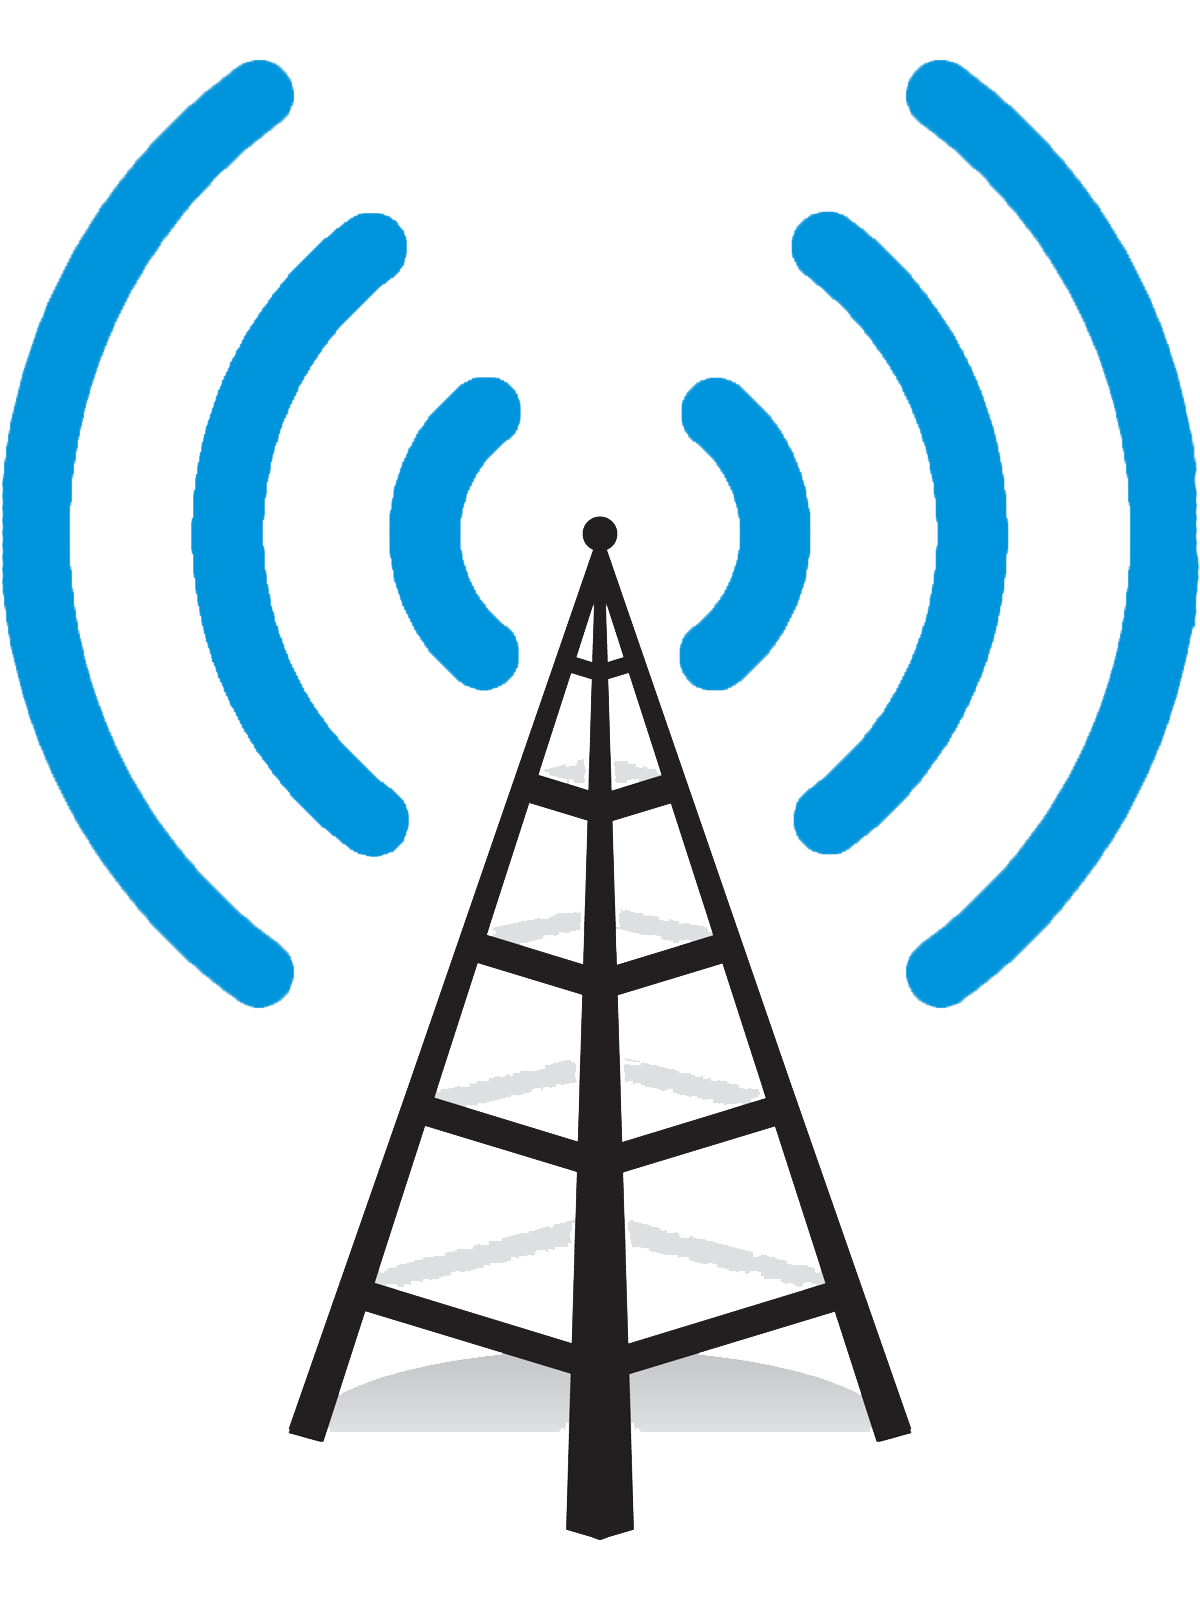
\includegraphics[width = 1cm]{rrh.png}};
   \node[below] at (r1.south) {RRH};
  \node (r2) at (0,4) {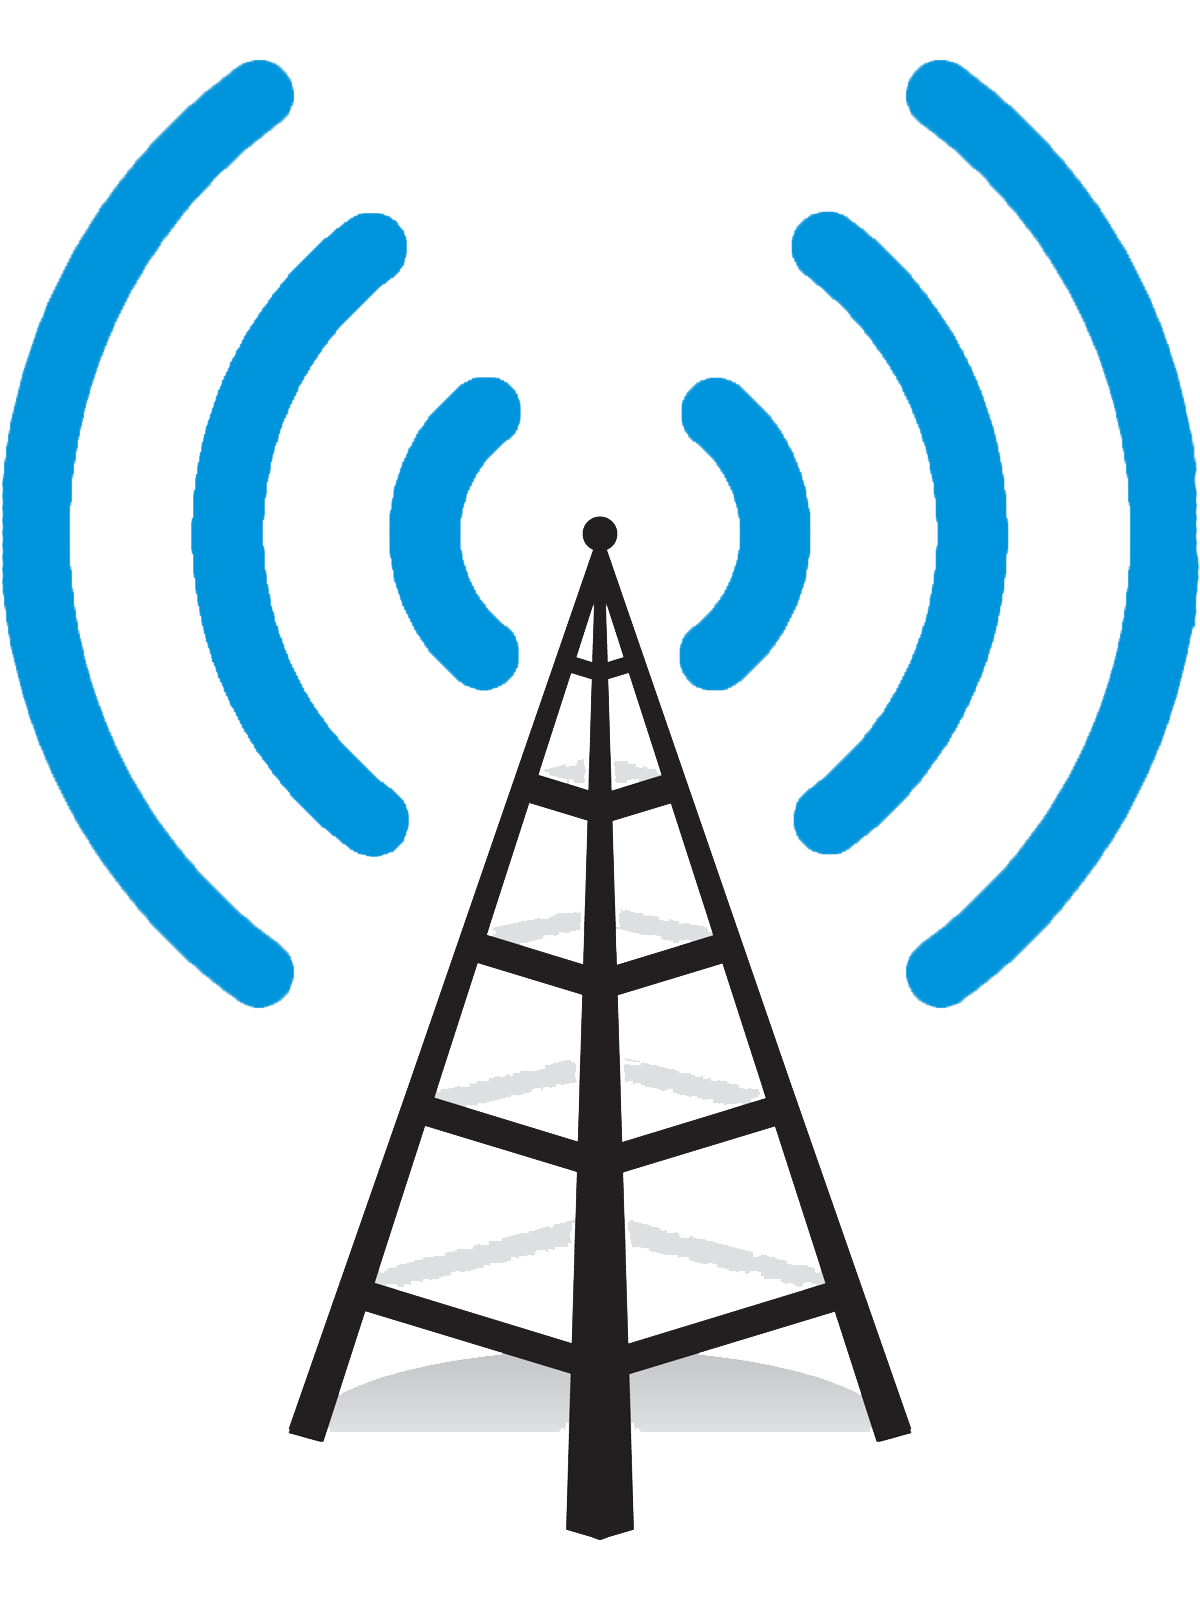
\includegraphics[width = 1cm]{rrh.png}};
   \node[below] at (r2.south) {RRH};
   \node (b1) at (12,0) {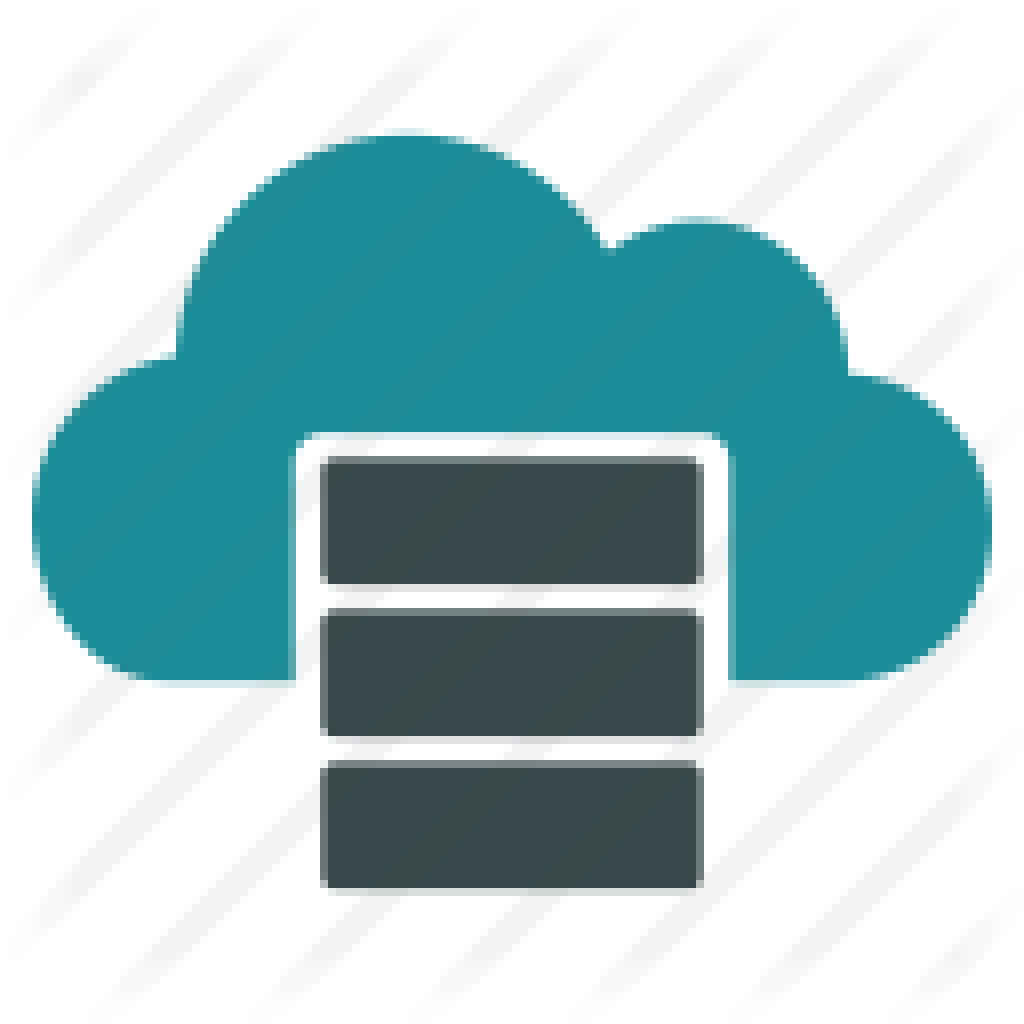
\includegraphics[width = 1cm]{bbu.png}};
   \node[below] at (b1.south) {BBU};
   \node (b2) at (12,4) {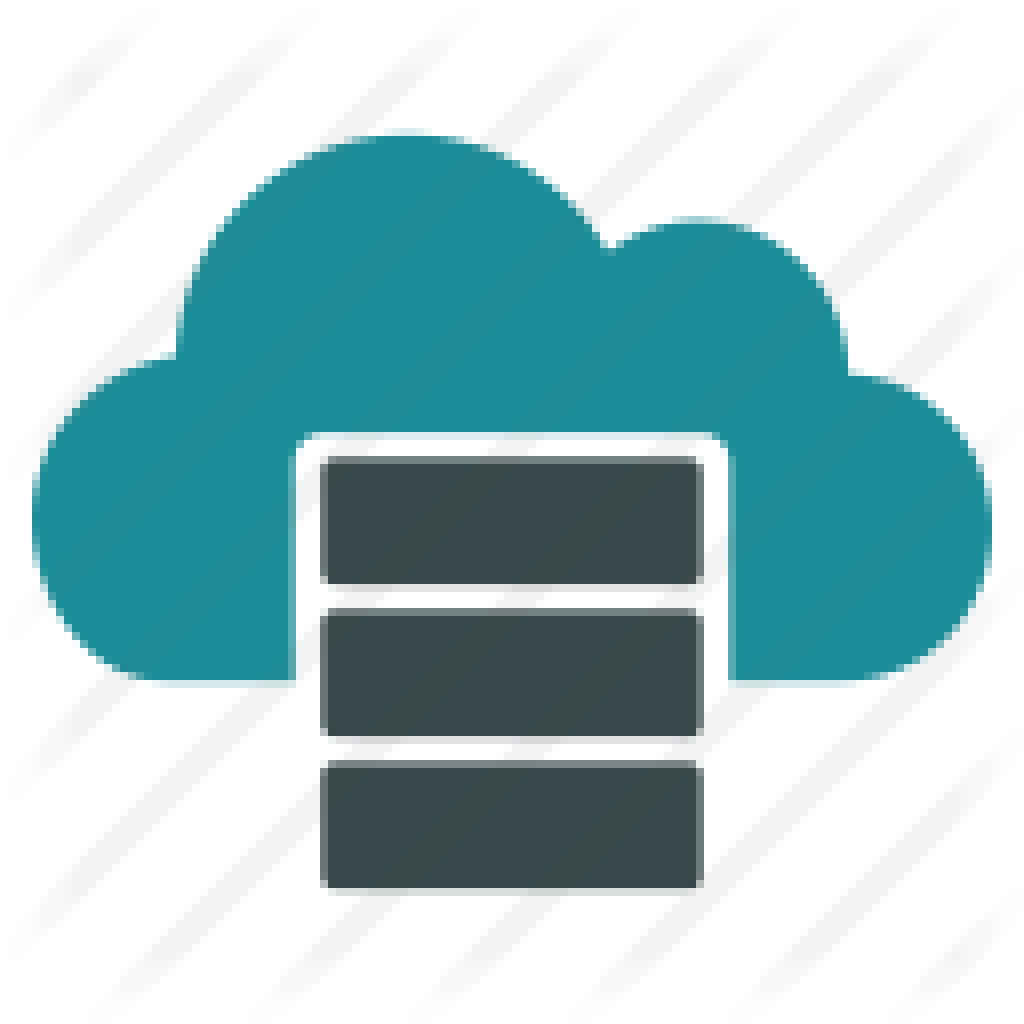
\includegraphics[width = 1cm]{bbu.png}};
	\node[below] at (b2.south) {BBU};
   \node (s1) at (4,2) {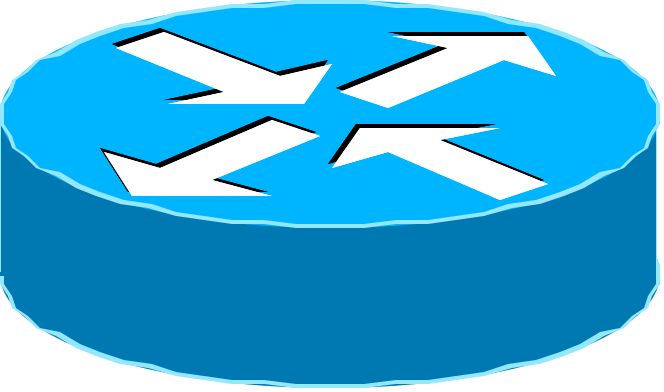
\includegraphics[width = 1cm]{switch.png}};
   \node (s2) at (8,2) {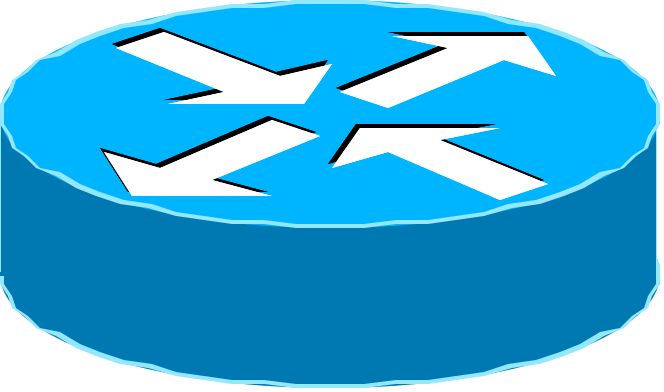
\includegraphics[width = 1cm]{switch.png}};
  
   \node (c) at (6,6) {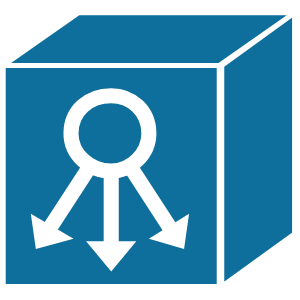
\includegraphics[width = 1cm]{controller.png}};
   	\node[right] at (c.north east) {Controller};

   	\node (rect) at (6,10) [draw,thick,minimum width=2cm,minimum height=1cm] {Algorithms};

\path (r1) edge [<->]  (s1);
\path (r2) edge [<->]  (s1);
\path (s2) edge [<->]  (s1);
\path (s2) edge [<->]  (b1);
\path (s2) edge [<->]  (b2);
\path (s2) edge [<->]  (c);
\path (s1) edge [<->]  (c);
\path (r1) edge [<->]  (c);
\path (r2) edge [<->]  (c);
\path (b1) edge [<->]  (c);
\path (b2) edge [<->]  (c);
\path (rect) edge [<->]  (c);


\end{tikzpicture}
}


 \caption{A TSN network managed by a controller, able to collect network informations, and control the nodes behavior.}

\label{fig:networkcontroller}
\end{center}
\end{figure}

\paragraph{Individual management of flows}

Standard 802.1Qbv~\cite{8613095} allows us to manage different flows in the nodes by a gate mechanism. The switch follows a routine that organize the sending time of flows on each output ports. To do so, the switch needs a Gate Control List (GCL). This GCL is computed by the user, and sent to each switch of the network by the controller. It is a list of dates, and for every date of the list are specified the output ports (gates) of the switch which are open or close.


Figure~\ref{fig:tsnqbv} from~\cite{durr2016no} shows the mechanism of a switch using 802.1Qbv technology. Considering a given period ($T_{cycle}$ in the figure), the switch selects at each time ($T_1 , T_2 , \ldots$ the queues that must be open to transmit packets. In figure~\ref{fig:tsnqbv}, at time $T_1$, all gates except the one for scheduled traffic are open, at time $T_2$, all gates are closed and at time $T_3$ only the gate for scheduled traffic is open.

  \begin{figure}
  \begin{center}
  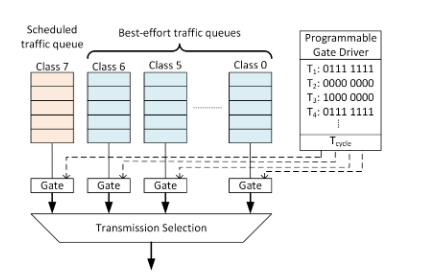
\includegraphics[width=0.8\textwidth]{Chapitre1/tsnqbv.png}
  \end{center}
  \caption{IEEE 802.1Qbv mechanism}\label{fig:tsnqbv}
  \end{figure}
      
With such a mechanism, it is possible to organize the flows in order to control the latency. The CGL are computed upstream considering the traffic (size of the datagrams, periodicity, or average data flow of each flow for non deterministic traffic). Several works on Time Aware Shaping have been developed on this topic: \cite{al2017modeling} introduce how to manage one deterministic flow and one best effort flow (non periodic generation of data, stochastic model). This paper shows that by correctly setting the GCL of the nodes, it is possible to ensure no contention for one deterministic flow. Nevertheless, works about managing several deterministic flows together are mainly based on linear programing~\cite{steiner2018traffic,silviu2017,nayak2017incremental,naresh2016}, which has an high complexity and does not scale well with number of routes and contention depth of the networks.

\paragraph{Synchronization}
To be efficient, the components of the network must be completely synchronized. Such an hypothesis seems unrealistic. Standards likes IEEE 802.1AS~\cite{5741898}, or IEEE 1588~\cite{4579760} propose good solutions for clock synchronization, but this problem is still difficult to solve. Indeed, even if those protocols propose good solution to re-synchronize clocks, there is still some offset between the clocks of the switch since it is impossible to ensure the length of a link between two components. This value can be deduced of the travel time of packets between two switches but this value highly depends of several factors, like the temperature of the link for example. Network designers use {\em Guard Time} to prevent this problem. The GCL are computed such that a gate is open before and after the theoretical arrival of packets. Such a mechanism induce artificial additional use of bandwidth, because a gate is open more than it should be.

\subsection{Limits of TSN when managing Deterministic flows}

All those standards are designed for a statistical management of the flows. In this thesis, we work on deterministic flows: our models and algorithms are not designed for a statistical approach like current traffic shaping, but a deterministically approach. We compute the exact date at which each flow is able to reach each node, without loss of bandwidth due to guard time. Furthermore, a statistical approach does not allow to control the contention and the exact forwarding time of the datagram in the network. This induce that a datagram sent periodically will not always have the same latency over a network. The variation of the latency is called \textbf{jitter}. The jitter is an indicator of the stability of the network. The higher the jitter, the higher the maximal value of the latency is.

Such an approach requires to rethink about our vision of the network management. We need the nodes to be perfectly synchronized otherwise it could be counter productive. Indeed, if a packet of a flow arrives in a node before or after the planned date, the gate is close and the packet is buffered, that induces additional latency.

Also, switches operation on the physical layer of the network induce an additional latency due to physical buffering. In store-and-forward concept~\cite{tindell1992store}, packets are stored at reception of a node before being forwarded. However, solution like cut-through~\cite{kermani1979virtual} allow to reduce storage size and corresponding delay to the header size only. But this is effective if the egress port is available to forward the packet at the same time only. If not, the packet is buffered until the port is free. Even if it is possible to adapt our model to take into consideration the physical buffering cost, it still induce additional latency, which is not desirable.

Next section present a new kind of switch, called Hyper-TSN switch, and that allows to override all the above limits.

\section{Deterministic management for a deterministic latency}
\label{sec:platform}


Most of the works developed around Deterministic Networking are still based on stochastic laws. Indeed, deterministic networking aims to ensure an upper bound on latency. Here, we propose to reduce the additional latency due to contention buffers at its minimum, and to remove jitters in network, which is a deeper aspect of deterministic networking.
Here, because of our desire to manage deterministic flows, multiple standards of TSN are not useful yet. Indeed, since the exact date of arrival of all packets are computed, we can get rid of several tools designed to manage the traffic on a statistical manner. 

We present in this section an Hyper-TSN switch that solves all the problematic of TSN when managing deterministic traffic.
This technology is under an advanced phase of research, and a prototype has been experimented in Nokia Bell Labs~\cite{guiraudleclercmarce2021}

\subsection{Hyper-TSN switch}


A 2x2 Hyper-TSN switch has been developed. It is composed of a switching matrix connected to a deterministic scheduler and two 10 Gbps ethernet 2 ways transceivers. The switching matrix includes also a monitoring circuitry. The deterministic scheduler controls the switching matrix and is configured with a timing table. This table is similar to a 802.1 Qbv Gate Control List (GCL). It defines the periodicity of the scheduling and, for each egress ports, the planed date of arrival of the frames which are part of deterministic flows. At each of these dates the deterministic scheduler sets the switching matrix to transmit data incoming on a specified ingress port. Figure~\ref{fig:schedulehtsn} shows an example of scheduling for deterministic and stochastic traffic.
 In such a switch, the buffers are totally removed: when a datagram arrives in the switch, it is instantly switched to the egress port, and there is no processing operation. This process allows us to reduce the physical delay to its lowest for scheduled traffic, while it is still possible to buffer the Best Effort traffic, which has not critical latency constraints.
\begin{center}

\begin{figure}[h]
  \centering
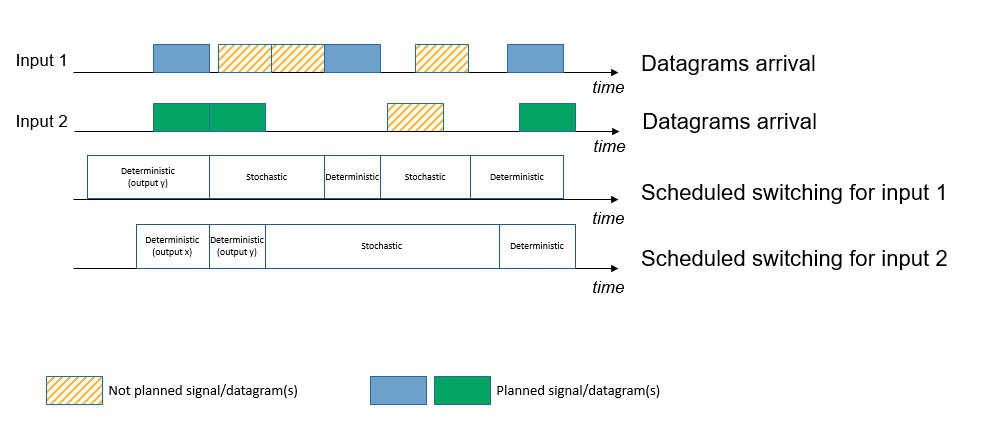
\includegraphics[scale=0.4]{Chapitre7/schedulerhypertsn.png}
\caption{ The scheduling of a 2x2 switch on which both deterministic and stochastic traffics arrives. The deterministic traffic is forwarded without contention.}
\label{fig:schedulehtsn}
\end{figure}
\end{center}

Hyper-TSN considers the flow as a reference~\cite{leclerc2020optical}. Since the exact arrival time of a datagram is known, if this latter arrives before or after the expected date, this means the physical delay between the sender of the datagram and the switch known by the controller is false. The monitoring circuitry of the switch detects this issue and an alert signal is sent to the controller that is able to reschedule correctly the GCL.
This vision solves the synchronization problem between the nodes, and is possible because the switches are developed on components with very precise clocks (Xilinx FPGA boards : Zynq UltraScale MPSoC zcu102,Zynq-7000 SoC zc706). 
The switch also includes a frame analyzer that enables to check that the switched frames are not corrupted and none is missing.

\subsection{Implementation and reliability tests}

To perform experiments, a generator of deterministic flows has been developed. This generator set the dates it sends the frames according to the controls received from the monitoring circuitry. The period are defined in the timing table. The size of the frames is set to fully load the ethernet links (ie $100\%$ load).
When starting, the monitoring circuitry detects that frames do not arrive at the planed date and sends control commands to the generator. These first frames are lost. Once the generator has rightly offset the dates it sends the frames, no more shifting has been performed during the running 2 hours experiment. $100\%$ of the frames are correctly switched without being corrupted or lost. The switching of each frame from the ingress port to the planed egress port is performed introducing only one clock cycle delay (here 3,87 ns).
Figure~\ref{fig:hypertsnswitch} shows the Hyper-TSN 2x2 switch developed and on which experiments was made.
\begin{center}

\begin{figure}[h]
  \centering
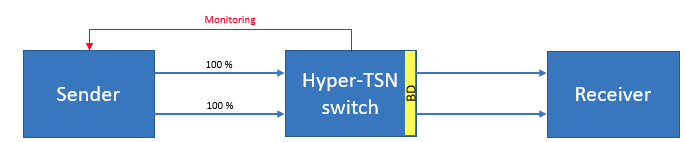
\includegraphics[scale=0.4]{Chapitre7/switchhypertsn.png}
\caption{ An Hyper-TSN switch with a 2x2 switching matrix.}
\label{fig:hypertsnswitch}
\end{figure}
\end{center}
